\chapter{कोशिका-चक्र का नियंत्रण और क्रमादेशित कोशिका-मृत्यु}\label{ch:b3:cell-cycle-apoptosis}

आपके शरीर की लगभग सौ अरब कोशिकाएँ आज जान-बूझकर मरेंगी, और सौ अरब उनकी
जगह लेने जन्मेंगी; आपकी आँत की भीतरी परत हर पाँच दिन में नई हो जाती है,
और आपकी लाल कोशिकाएँ हर चार महीने में। कोई मेंढकछौना बिना रक्त बहे अपनी
पूँछ खो देता है; किसी मानव भ्रूण की उँगलियों के बीच की झिल्ली आठवें
सप्ताह में लुप्त हो जाती है; किसी मस्तिष्क में कभी बने न्यूरॉनों में से
आधे जन्म से पहले मार दिए जाते हैं। इनमें से हर मृत्यु कोशिका स्वयं किसी
कार्यक्रम पर निष्पादित करती है, और हर जन्म को कोई नियंत्रण-तंत्र
अनुज्ञा देता है जो चक्र के दो-तीन बिंदुओं पर तय करता है कि कोशिका आगे
बढ़ सकती है या नहीं। ये दो कार्यक्रम --- विभाजन और आत्महत्या --- इस
अध्याय का विषय हैं। वे खमीर, मेंढक के अंडों, समुद्री साही और ऐसे कृमि
में सुलझाए गए जिसमें ठीक $1090$ कायिक कोशिकाएँ हैं जिनमें से ठीक $131$
मरती हैं, और वे मनुष्यों में वही निकले, जहाँ उनकी विफलताएँ एक ओर कर्कट
हैं और दूसरी ओर अपह्रास।

\section{चक्र का इंजन}

\begin{definition}[चक्रिन और चक्रिन-निर्भर काइनेज़]\label{def:b3:cell-cycle-apoptosis:cdk}
\index{चक्रिन}\index{चक्रिन-निर्भर काइनेज़}\index{पश्चावस्था-प्रवर्तक संकुल}\index{कोशिका-चक्र}
कोशिका-चक्र --- G1, S (प्रतिकृति), G2, M (समसूत्री विभाजन) --- को
प्रोटीन काइनेज़ों का एक कुल चलाता है, यानी \emph{चक्रिन-निर्भर काइनेज़}
(CDK), जिनकी उत्प्रेरक उपइकाइयाँ पूरे चक्र में मौजूद रहती हैं पर सक्रिय
तभी होती हैं जब वे किसी \emph{चक्रिन} से बँधी हों, यानी ऐसी नियामक
उपइकाई से जिसकी सांद्रता एक नियत क्रम में उठती और गिरती है: वृद्धि
कारकों की अनुक्रिया में G1 में Cdk4/6 के साथ चक्रिन D, G1/S संक्रमण पर
Cdk2 के साथ चक्रिन E, S भर Cdk2 के साथ चक्रिन A, और समसूत्री विभाजन में
प्रवेश पर Cdk1 के साथ चक्रिन B। हर चक्रिन--CDK अपनी प्रावस्था के
प्रोटीनों का फ़ॉस्फ़ोरिलन करता है --- प्रतिकृति के उद्गम, लैमिन,
कंडेंसिन, तर्कु-संयोजन के एंज़ाइम --- और हर एक अपने चक्रिन के विनाश से
बंद होता है: यूबिक्विटिन लाइगेज़ (G1/S में SCF, समसूत्री विभाजन में
\emph{पश्चावस्था-प्रवर्तक संकुल}, APC/C) चक्रिनों को प्रोटिएज़ोम के लिए
अंकित कर देती हैं। Cdk1 की क्रियाशीलता पर एक और द्वार है: काइनेज़ Wee1
द्वारा लगाया और फ़ॉस्फ़ेटेज़ Cdc25 द्वारा हटाया जाने वाला कोई निरोधी
फ़ॉस्फ़ोरिलन, और ऐसे छोटे निरोधक प्रोटीन (p21, p27, p16) जो संकुलों से
बँध जाते हैं। इस तरह चक्र काइनेज़-लहरों का एक क्रमित अनुक्रम है, और हर
लहर का अंत उसी के प्रोटीन-अपघटन में होता है जिसने उसे पैदा किया।
\end{definition}

\begin{proof}[प्रमाण-सामग्री]
तीन धाराएँ आकर मिलीं। हार्टवेल (1970 के दशक) ने मुकुलक खमीर के
ताप-संवेदी \emph{cdc} उत्परिवर्ती अलग किए, जिनमें से हर एक किसी एक
अवस्था पर एक अभिलाक्षणिक कली-आकार के साथ रुका था, और उन्होंने
\emph{Start} परिभाषित किया, यानी G1 का वह बिंदु जिसके बाद कोई कोशिका
किसी चक्र के लिए प्रतिबद्ध हो जाती है। नर्स (1980 के दशक) ने विखंडन
खमीर में पाया कि \emph{cdc2} समसूत्री विभाजन का समय तय करता है और यह
कि मानव जीन, खमीर में डालने पर, उत्परिवर्ती को उबार लेता है: वह काइनेज़
Cdk1 थी, जो खमीर से मनुष्य तक संरक्षित है। हंट (1983) ने समुद्री साही
के अंडों में ऐसा प्रोटीन पाया जो हर चक्र भर जमा होता था और हर विभाजन पर
अचानक नष्ट हो जाता था, और उसे \omterm{def:b3:cell-cycle-apoptosis:cdk}{चक्रिन} कहा। इस बीच मेंढक के अंडे से कोई
``परिपक्वन-प्रवर्तक कारक'' मिला था जो किसी भी केंद्रक को समसूत्री
विभाजन में धकेल देता था; वह Cdk1 से बँधा \omterm{def:b3:cell-cycle-apoptosis:cdk}{चक्रिन} B था। राव और जॉनसन
(1970) ने कोशिकाओं को संलयित करके दिखाया था कि कोई S-प्रावस्था कोशिका
किसी G1 केंद्रक को प्रतिकृति में धकेल देती है, जबकि कोई G2 केंद्रक
प्रतीक्षा करता है --- संकेत कोशिकाद्रव्य ढोता है, और जो केंद्रक प्रतिकृत
हो चुका हो उससे फिर प्रतिकृति नहीं कराई जा सकती।
\end{proof}

\begin{omfigure}
\begin{tikzpicture}[every node/.style={font=\scriptsize}, >=stealth]
  % cycle circle with phases
  \draw[very thick, omDef!50] (0,0) circle (2.2);
  \foreach \a/\b/\col/\lab/\r in {90/200/omDef!25/G1/1.55, 200/270/omProp!30/S/1.55, 270/315/omMeth!30/G2/1.55, 315/450/omThm!30/M/1.55} {
    \fill[\col] (0,0) -- (\a:2.2) arc[start angle=\a, end angle=\b, radius=2.2] -- cycle;
    \node[font=\small\bfseries] at ({(\a+\b)/2}:\r) {\lab};
  }
  \fill[white] (0,0) circle (1.0);
  \draw[very thick, omDef!50] (0,0) circle (2.2);
  % cyclin-CDK labels around
  \node[left, align=right] at (-2.4,1.2) {चक्रिन D--Cdk4/6\\वृद्धि कारक, Rb बंद};
  \node[left, align=right] at (-2.4,-1.0) {चक्रिन E--Cdk2\\उद्गम चलते हैं};
  \node[anchor=north east, align=right] at (-1.3,-2.2) {चक्रिन A--Cdk2\\प्रतिकृति};
  \node[right, align=left] at (2.4,-1.0) {चक्रिन B--Cdk1\\समसूत्री विभाजन में प्रवेश};
  \node[right, align=left] at (2.4,1.3) {APC/C चक्रिन B और सेक्युरिन\\नष्ट करता है: पश्चावस्था, निकास};
  % checkpoints as bars
  \foreach \a in {160,270,20} \draw[very thick, omThm] (\a:1.95) -- (\a:2.45);
  \node[align=center, anchor=south east] at (-1.2,2.35) {निर्बंधन बिंदु:\\वृद्धि कारक हैं?};
  \node[align=left, anchor=west] at (2.55,0.35) {तर्कु जाँच-बिंदु:\\सारे गुणसूत्रबिंदु जुड़े?};
  \node[align=center, anchor=north] at (1.5,-2.55) {G2/M जाँच-बिंदु:\\DNA अक्षत है?};
  \draw[->, thick] (0,0) ++(60:1.25) arc[start angle=60, end angle=30, radius=1.25];
\end{tikzpicture}

{\small चक्रिन--CDK लहरों के अनुक्रम के रूप में चक्र, जिसमें हर लहर
अपने \omterm{def:b3:cell-cycle-apoptosis:cdk}{चक्रिन} के विनाश से समाप्त होती है, और तीनों \omterm{def:b3:cell-cycle-apoptosis:checkpoints}{जाँच-बिंदु} (लाल
पट्टियाँ) जहाँ कोशिका पूछती है कि आगे बढ़ना है या नहीं।}
\end{omfigure}

\begin{theorem}[एक स्विच और एक विलंबित ब्रेक मिलकर दोलक बनाते हैं]\label{thm:b3:cell-cycle-apoptosis:oscillator}
\index{शिथिलन दोलक}\index{द्विस्थायित्व!कोशिका-चक्र}\index{शैथिल्य}
मान लीजिए $A$ \omterm{def:b3:cell-cycle-apoptosis:cdk}{चक्रिन} B--Cdk1 की क्रियाशीलता है और $C$ \omterm{def:b3:cell-cycle-apoptosis:cdk}{चक्रिन}
B की मात्रा। मानिए कि (i) किसी नियत $C$ के लिए $A$ तेज़ी से ऐसी स्थायी
अवस्था पर आ जाता है जो किसी धन पुनर्भरण के ज़रिए $C$ पर निर्भर है
(सक्रिय Cdk1 अपने सक्रियक Cdc25 को सक्रिय करता है और अपने निरोधक Wee1
को रोकता है), जिससे स्थायी-अवस्था वक्र $A^{*}(C)$ S-आकार का है: दो
ऐसे $C$ के लिए जो दो देहलियों $C_{1} < C_{2}$ के बीच हो, एक निम्न और एक उच्च
दोनों अवस्थाएँ होती हैं, और तंत्र उसी शाखा पर बना रहता है जिस पर वह है
(\emph{शैथिल्य}); (ii) $C$ धीरे बदलता है, अचर दर $k_{s}$ से संश्लेषित
होता है और APC/C के ज़रिए दर $k_{d}A\,C$ से अपघटित, जिसे सक्रिय Cdk1
कुछ विलंब के बाद चालू कर देता है। तब तंत्र की कोई स्थिर स्थायी अवस्था
नहीं होती और वह कोई \emph{शिथिलन दोलन} करता है: $C$ निम्न शाखा पर तब तक
जमा होता है जब तक वह $C_{2}$ पार न कर ले, $A$ उच्च शाखा पर कूद जाता है
(समसूत्री प्रवेश), अपघटन संश्लेषण से आगे निकल जाता है और $C$ तब तक
गिरता है जब तक वह $C_{1}$ पार न कर ले, $A$ निम्न शाखा पर ढह जाता है
(समसूत्री निकास), और चक्र दोहरा जाता है। आवर्तकाल मुख्यतः धीमे चर से तय
होता है: उठान के लिए लगभग $C_{2}/k_{s}$, और उसके साथ
$C_{2}$ से $C_{1}$ तक अपघटित होने का समय।
\end{theorem}
\begin{proof}[आंशिक प्रमाण]
इस युग्म की किसी स्थायी अवस्था के लिए $\mathrm{d}C/\mathrm{d}t = 0$
चाहिए होगा, यानी $k_{s} = k_{d}A^{*}(C)\,C$, S-आकार वक्र के किसी बिंदु
पर। निम्न शाखा पर $A^{*}$ छोटा है, इसलिए
$k_{d}A^{*}C < k_{s}$ रहता है, उस $C$ के लिए जो $C_{2}$ तक हो: \omterm{def:b3:cell-cycle-apoptosis:cdk}{चक्रिन} उठता है, और तंत्र शाखा के
सिरे से बाहर ले जाया जाता है। उच्च शाखा पर $A^{*}$ बड़ा है, इसलिए
$k_{d}A^{*}C > k_{s}$ रहता है, उस $C$ के लिए जो नीचे $C_{1}$ तक हो: \omterm{def:b3:cell-cycle-apoptosis:cdk}{चक्रिन}
गिरता है, और तंत्र उस सिरे से बाहर ले जाया जाता है। एकमात्र संभावित
स्थायी अवस्था बीच की, अस्थिर शाखा पर पड़ती, और वहाँ का कोई बिंदु
प्रतिकर्षित करता है; इसलिए कोई स्थिर स्थायी अवस्था नहीं है, और
प्रक्षेपपथ, जो दोनों स्थिर शाखाओं और उनके बीच की छलाँगों तक सीमित है,
चक्र लगाता है। निम्न शाखा पर समय
$\int \mathrm{d}C/(k_{s} - k_{d}A^{*}C) \approx C_{2}/k_{s}$ है जब
$A^{*}$ छोटा हो, और उच्च शाखा पर समय वह छोटा समय है जिसमें
$C_{2} - C_{1}$ दर $k_{d}A^{*}_{\text{उच्च}}C$ से अपघटित होता है।
Cdc25/Wee1 पुनर्भरण से S-आकार वक्र का होना यहाँ मान लिया गया है; वह
वही द्विस्थायित्व है जो वर्ष~2 के खंड के स्वयं-सक्रियकारी जीन का है,
जिसमें अब तेज़ चर कोई काइनेज़ है और धीमा उसका \omterm{def:b3:cell-cycle-apoptosis:cdk}{चक्रिन}।
\end{proof}

\begin{omfigure}
\begin{tikzpicture}
\begin{axis}[
  width=6.6cm, height=5.6cm,
  axis lines=left,
  xmin=0, xmax=1.4, ymin=0, ymax=1.1,
  xlabel={चक्रिन B, $C$}, ylabel={Cdk1 क्रियाशीलता, $A$},
  xlabel style={font=\small, at={(axis description cs:0.5,-0.12)}, anchor=north}, ylabel style={font=\small},
  tick label style={font=\scriptsize}, xtick={0.4,1.0}, xticklabels={$C_{1}$,$C_{2}$}, ytick=\empty,
  clip=false,
]
% S-shaped nullcline: two stable branches and a dashed unstable one
\addplot[very thick, omDef, smooth] coordinates {(0,0.02) (0.5,0.04) (0.9,0.07) (1.0,0.1)};
\addplot[very thick, omDef, dashed, smooth] coordinates {(1.0,0.1) (0.85,0.3) (0.7,0.5) (0.55,0.7) (0.4,0.9)};
\addplot[very thick, omDef, smooth] coordinates {(0.4,0.9) (0.6,0.94) (1.0,0.97) (1.4,0.98)};
\draw[->, very thick, omThm] (axis cs:0.05,0.15) -- (axis cs:0.98,0.15);
\draw[->, very thick, omThm] (axis cs:1.04,0.18) -- (axis cs:1.04,0.82);
\draw[->, very thick, omThm] (axis cs:0.98,0.84) -- (axis cs:0.42,0.84);
\draw[->, very thick, omThm] (axis cs:0.36,0.82) -- (axis cs:0.36,0.18);
\node[font=\scriptsize, omThm, anchor=south west] at (axis cs:0.36,0.24) {चक्रिन जमा होता है};
\node[font=\scriptsize, omThm, anchor=west] at (axis cs:1.07,0.5) {प्रवेश};
\node[font=\scriptsize, omThm, anchor=south] at (axis cs:0.7,1.0) {APC/C चक्रिन अपघटित करता है (समसूत्री विभाजन)};
\node[font=\scriptsize, omThm, anchor=east] at (axis cs:0.33,0.5) {निकास};
\node[font=\scriptsize, omDef, anchor=north east] at (axis cs:1.38,0.95) {$A^{*}(C)$};
\end{axis}
\begin{axis}[
  at={(7.6cm,0)}, anchor=south west,
  width=6.6cm, height=5.6cm,
  axis lines=left,
  xmin=0, xmax=3, ymin=0, ymax=1.2,
  xlabel={समय (चक्र)}, ylabel={},
  xlabel style={font=\small, at={(axis description cs:0.5,-0.12)}, anchor=north},
  tick label style={font=\scriptsize}, xtick={0,1,2,3}, ytick=\empty,
  clip=false,
]
\addplot[very thick, omDef] coordinates {(0,0.4) (0.8,1.0) (0.95,0.4) (1.75,1.0) (1.9,0.4) (2.7,1.0) (2.85,0.4) (3,0.5)};
\addplot[very thick, omThm] coordinates {(0,0.05) (0.8,0.05) (0.8,0.95) (0.95,0.95) (0.95,0.05) (1.75,0.05) (1.75,0.95) (1.9,0.95) (1.9,0.05) (2.7,0.05) (2.7,0.95) (2.85,0.95) (2.85,0.05) (3,0.05)};
\node[font=\scriptsize, omDef, anchor=south west] at (axis cs:1.0,0.1) {चक्रिन B};
\node[font=\scriptsize, omThm, anchor=south west] at (axis cs:1.0,1.0) {Cdk1 क्रियाशीलता};
\end{axis}
\end{tikzpicture}

{\small बाएँ: दोलक का कला-समतल। S-आकार वक्र \omterm{def:b3:cell-cycle-apoptosis:cdk}{चक्रिन} के हर स्तर के लिए
Cdk1 की तेज़ स्थायी अवस्था है; लाल पाश ही चक्र है --- निम्न शाखा पर
धीमा जमाव, $C_{2}$ पर एक छलाँग, उच्च शाखा पर तेज़ अपघटन, और
$C_{1}$ पर वापसी की छलाँग। दाएँ: इससे बनने वाला काल-क्रम, यानी \omterm{def:b3:cell-cycle-apoptosis:cdk}{चक्रिन}
का एक आरादंती वक्र और काइनेज़ की एक वर्ग-तरंग।}
\end{omfigure}

\begin{example}[मेंढक का अंडा घड़ी क्यों है]\label{ex:b3:cell-cycle-apoptosis:frog}
कोई निषेचित मेंढक-अंडा छह घंटों में बारह बार विभाजित होता है, बिना किसी
वृद्धि, बिना किसी अनुलेखन और बिना किसी \omterm{def:b3:cell-cycle-apoptosis:checkpoints}{जाँच-बिंदु} के,
\qty{30}{min} के अंतरालों पर: वह प्रमेय का दोलक नंगा चलता हुआ है, और
उसके कोशिकाद्रव्य का कोई निष्कर्ष परखनली में भी चक्र लगाता रहता है,
जिसमें \omterm{def:b3:cell-cycle-apoptosis:cdk}{चक्रिन} उठता-गिरता है और विभाजित करने को कुछ भी नहीं होता। कोई
अनअपघट्य \omterm{def:b3:cell-cycle-apoptosis:cdk}{चक्रिन} B जोड़ देने पर निष्कर्ष समसूत्री विभाजन में बंद हो जाता
है, क्योंकि $C$ कभी $C_{1}$ से नीचे नहीं गिर सकता; चक्रिन-संश्लेषण
रोकने पर वह अंतरावस्था में बंद हो जाता है। किसी कायिक कोशिका में वही
इंजन अगले खंड के नियंत्रणों में लिपटा है, जो उसे देहलियों पर तब तक थामे
रखते हैं जब तक शर्तें पूरी न हों, जिससे आवर्तकाल आधे घंटे के बजाय एक दिन
बन जाता है और अनिश्चित काल तक लंबा हो सकता है।
\end{example}

\section{जाँच-बिंदु}

\begin{definition}[जाँच-बिंदु]\label{def:b3:cell-cycle-apoptosis:checkpoints}
\index{जाँच-बिंदु}\index{निर्बंधन बिंदु}\index{तर्कु-संयोजन जाँच-बिंदु}\index{प्रतिकृति-अनुज्ञापन}
कोई \emph{जाँच-बिंदु} ऐसा नियंत्रण है जो किसी संक्रमण पर चक्र को तब तक
रोक देता है जब तक कोई शर्त पूरी न हो, और वह इंजन पर काम करके ऐसा करता
है --- किसी CDK या किसी यूबिक्विटिन लाइगेज़ को रोककर। तीन सबसे अधिक
मायने रखते हैं। पछेती G1 में \emph{निर्बंधन बिंदु} (खमीर में Start):
कोशिका तभी आगे बढ़ती है जब वृद्धि कारक, पोषक और आकार अनुमति दें; उसके
आगे चक्र उनके बिना ही पूरा हो जाता है। \emph{G2/M जाँच-बिंदु}:
क्षतिग्रस्त या अप्रतिकृत DNA, जिसका संकेत
\cref{ch:b3:dna-repair} की \omterm{def:b3:dna-repair:ddr}{ATM}/ATR काइनेज़ देती हैं, Cdc25 को निरुद्ध
रखता है और इस तरह Cdk1 को फ़ॉस्फ़ोरिलित तथा निष्क्रिय रखता है।
\emph{तर्कु-संयोजन जाँच-बिंदु}: \omterm{def:b3:cytoskeleton-motility:filaments}{सूक्ष्मनलिकाओं} से न जुड़ा कोई एक भी
गुणसूत्रबिंदु ऐसा विसरणशील निरोधक (Cdc20 से बँधा Mad2) बनाता है जो
APC/C को बंद रखता है, ताकि पश्चावस्था अंतिम गुणसूत्र की प्रतीक्षा करे।
चौथे नियंत्रण में कोई प्रतीक्षा-चरण नहीं है पर वह उतना ही कठोर है:
\emph{प्रतिकृति-अनुज्ञापन}। उद्गमों पर MCM हेलिकेज़ केवल G1 में लादी
जाती है, जब CDK क्रियाशीलता कम हो, और S प्रावस्था शुरू होते ही लादने
वाले कारक नष्ट या निरुद्ध कर दिए जाते हैं, ताकि हर उद्गम प्रति चक्र
केवल एक ही बार चले --- यही कारण है कि राव और जॉनसन के संलयनों में कोई
G2 केंद्रक फिर से प्रतिकृति नहीं कर सका।
\end{definition}

\begin{proposition}[निर्बंधन बिंदु एक स्विच है]\label{prop:b3:cell-cycle-apoptosis:rb}
\index{दृष्टिपटलार्बुद प्रोटीन}\index{E2F}
अगेती G1 में अनुलेखन-कारक \emph{E2F}, जो S प्रावस्था के जीन (\omterm{def:b3:cell-cycle-apoptosis:cdk}{चक्रिन} E,
\omterm{def:b3:cell-cycle-apoptosis:cdk}{चक्रिन} A, प्रतिकृति के एंज़ाइम) चलाता है, \emph{\omterm{prop:b3:cell-cycle-apoptosis:rb}{दृष्टिपटलार्बुद
प्रोटीन}} Rb द्वारा निष्क्रिय रखा जाता है। वृद्धि कारक \omterm{def:b3:cell-cycle-apoptosis:cdk}{चक्रिन} D प्रेरित
करते हैं, और \omterm{def:b3:cell-cycle-apoptosis:cdk}{चक्रिन} D--Cdk4/6 Rb का फ़ॉस्फ़ोरिलन करने लगता है, जिससे
थोड़ा E2F मुक्त होता है; फिर E2F \omterm{def:b3:cell-cycle-apoptosis:cdk}{चक्रिन} E प्रेरित करता है, और \omterm{def:b3:cell-cycle-apoptosis:cdk}{चक्रिन}
E--Cdk2 Rb का कहीं अधिक फ़ॉस्फ़ोरिलन करता है --- एक धन पुनर्भरण जो, किसी
देहली के पार हो जाने पर, बिना और वृद्धि कारक के स्वयं पूरा हो जाता है।
कोशिका \omterm{def:b3:cell-cycle-apoptosis:checkpoints}{निर्बंधन बिंदु} पार कर चुकी है; E2F अपना ही जीन भी प्रेरित करता
है। Rb का ह्रास, या Cdk4/6 निरोधक p16 का, या \omterm{def:b3:cell-cycle-apoptosis:cdk}{चक्रिन} D का प्रवर्धन,
वृद्धि कारक की आवश्यकता पूरी तरह हटा देता है, और इनमें से हर एक कर्कट
में आम है (\cref{ch:b3:cancer-biology}); जो औषधें Cdk4/6 को रोकती हैं
वे अब उन स्तन-कर्कटों के विरुद्ध काम में ली जाती हैं जो इसी स्विच पर
निर्भर हैं।
\end{proposition}

\begin{omfigure}
\begin{tikzpicture}[every node/.style={font=\scriptsize}, >=stealth]
  \node[draw, thick, rounded corners, fill=omProp!25, minimum width=2.2cm] (gf) at (0,2.2) {वृद्धि कारक};
  \node[draw, thick, rounded corners, fill=omDef!20, minimum width=2.4cm] (cd) at (0,1.0) {चक्रिन D--Cdk4/6};
  \node[draw, thick, rounded corners, fill=omThm!20, minimum width=1.6cm] (rb) at (3.8,1.0) {Rb};
  \node[draw, thick, rounded corners, fill=omMeth!25, minimum width=1.6cm] (e2f) at (7.2,1.0) {E2F};
  \node[draw, thick, rounded corners, fill=omDef!20, minimum width=2.4cm] (ce) at (7.2,-0.6) {चक्रिन E--Cdk2};
  \node[draw, thick, rounded corners, fill=gray!15, align=center, minimum width=2.6cm] (s) at (10.8,1.0) {S-प्रावस्था जीन:\\चक्रिन A, MCM, \dots};
  \draw[->, thick] (gf) -- (cd);
  \draw[-|, thick, omThm] (cd) -- (rb) node[midway, above, font=\tiny] {फ़ॉस्फ़ोरिलित करता है};
  \draw[-|, thick, omThm] (rb) -- (e2f) node[midway, above, font=\tiny] {निष्क्रिय रखता है};
  \draw[->, thick] (e2f) -- (s);
  \draw[->, thick] (e2f) -- (ce) node[midway, right] {प्रेरित करता है};
  \draw[-|, thick, omThm] (ce.west) -- ++(-2.2,0) |- (rb.south) node[pos=0.25, below] {Rb का और फ़ॉस्फ़ोरिलन};
  \draw[->, thick, omMeth!70!black] (e2f.north) .. controls (6.0,2.2) and (6.8,2.2) .. (e2f.north east) node[pos=0.5, above] {अपना ही जीन प्रेरित करता है};
  \node[draw, thick, rounded corners, fill=omThm!10] (p16) at (0,-0.6) {p16}; \draw[-|, thick, omThm] (p16) -- (cd);
\end{tikzpicture}

{\small \omterm{def:b3:cell-cycle-apoptosis:checkpoints}{निर्बंधन बिंदु}। वृद्धि कारक Rb का फ़ॉस्फ़ोरिलन शुरू करते हैं,
जिससे थोड़ा E2F मुक्त होता है; E2F \omterm{def:b3:cell-cycle-apoptosis:cdk}{चक्रिन} E प्रेरित करता है, जिसकी
काइनेज़ Rb का और फ़ॉस्फ़ोरिलन करती है --- एक धन पुनर्भरण जो संक्रमण पूरा
कर देता है और उसे आरंभिक संकेत से स्वतंत्र बना देता है। पट्टियाँ
निरोध चिह्नित करती हैं।}
\end{omfigure}

\begin{proposition}[पश्चावस्था प्रोटीन-अपघटनी निर्णय है]\label{prop:b3:cell-cycle-apoptosis:anaphase}
\index{सेक्युरिन}\index{सेपरेज़}\index{कोहेसिन}
सहोदरी क्रोमैटिड S प्रावस्था से \emph{कोहेसिन} के वलयों द्वारा साथ
थामे रखे जाते हैं। मध्यावस्था पर, जब हर गुणसूत्रबिंदु जुड़ चुका हो और
तर्कु \omterm{def:b3:cell-cycle-apoptosis:checkpoints}{जाँच-बिंदु} चुप हो, APC/C अपने सक्रियक Cdc20 के साथ दो प्रोटीनों
का यूबिक्विटिनीकरण करता है: \omterm{def:b3:cell-cycle-apoptosis:cdk}{चक्रिन} B, जिसका ह्रास Cdk1 को निष्क्रिय कर
देता है और कोशिका को समसूत्री विभाजन से निकलने देता है, और
\emph{सेक्युरिन}, जिसका ह्रास प्रोटिएज़ \emph{सेपरेज़} को मुक्त कर देता
है, जो कोहेसिन काट देती है। सारे सहोदरी युग्म एक-दूसरे के सेकंडों के
भीतर अलग हो जाते हैं, तर्कु से ध्रुवों की ओर खिंचते हुए, और कोशिका
ऐक्टिन तथा \omterm{def:b3:cytoskeleton-motility:motors}{मायोसिन}~II के उस वलय से विभाजित होती है जो वहीं जुड़ता है
जहाँ तर्कु का मध्यक्षेत्र वल्कुट को (RhoA के ज़रिए) बताता है। यह निर्णय
इसलिए अनुत्क्रमणीय है कि वह प्रोटीन-अपघटनी है: कटा कोहेसिन फिर जोड़ा
नहीं जा सकता, और अपघटित \omterm{def:b3:cell-cycle-apoptosis:cdk}{चक्रिन} फिर से संश्लेषित करना पड़ता है। यहाँ की
त्रुटियाँ --- कोई गुणसूत्र गलत ध्रुव को खिंच जाना, कोई पश्चावस्था अंतिम
जुड़ाव से पहले शुरू हो जाना --- असुगुणित पुत्रियाँ पैदा करती हैं, जो
अर्बुदों की और गर्भपातों की सबसे आम गुणसूत्री असामान्यता है।
\end{proposition}

\begin{omfigure}
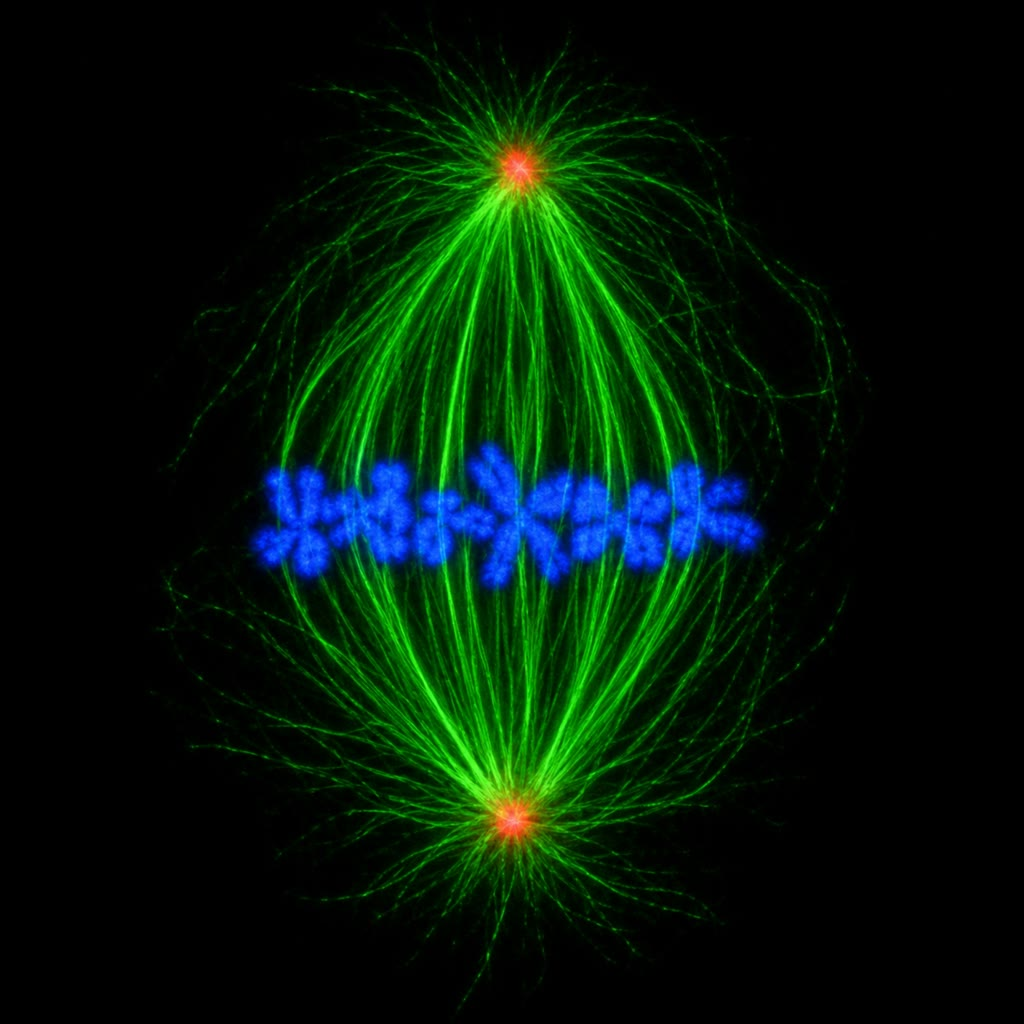
\includegraphics[width=0.36\linewidth]{images/book5/ai/b5-10-mitotic-spindle.jpg}\hspace{0.04\linewidth}
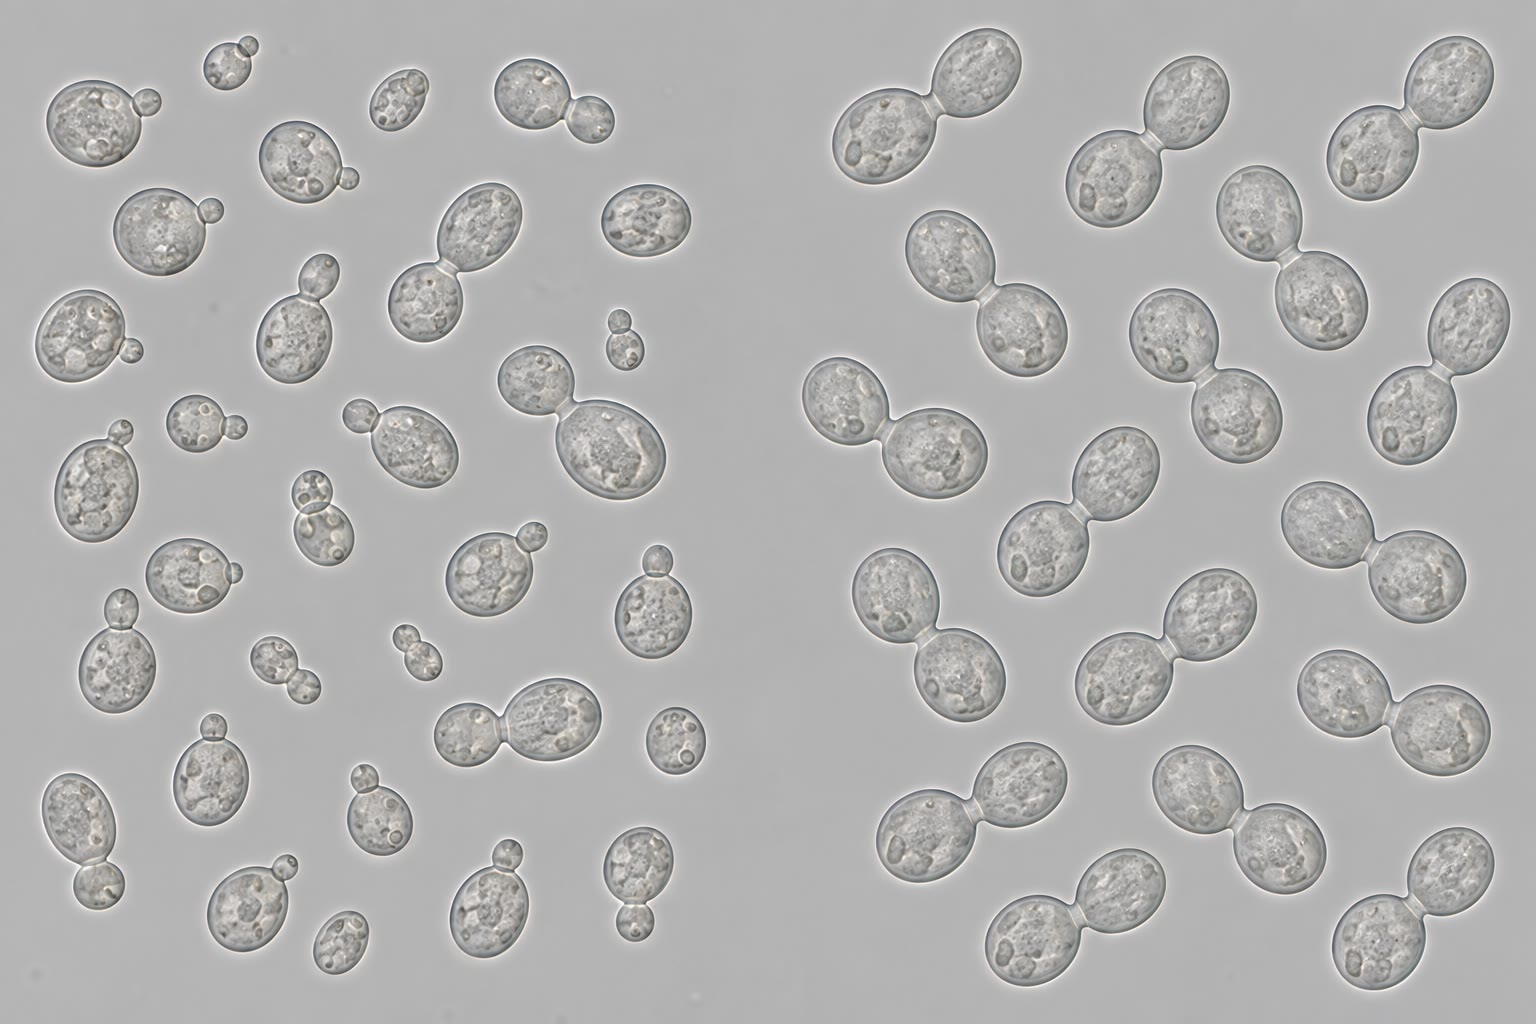
\includegraphics[width=0.54\linewidth]{images/book5/ai/b5-10-yeast-cdc-mutants.jpg}

{\small बाएँ: कोई मध्यावस्था कोशिका --- दोनों ध्रुवों (लाल) से तर्कु
\omterm{def:b3:cytoskeleton-motility:filaments}{सूक्ष्मनलिकाएँ} (हरी), पट्ट पर पंक्तिबद्ध गुणसूत्र (नीले), वही क्षण
जिस पर तर्कु \omterm{def:b3:cell-cycle-apoptosis:checkpoints}{जाँच-बिंदु} निर्णय करता है। दाएँ: मुकुलक खमीर,
वन्य-प्ररूप जिसमें हर आकार की कलियाँ हैं (बाएँ) और कोई \emph{cdc}
उत्परिवर्ती जिसमें हर कोशिका एक ही अवस्था पर रुकी है और हर एक की कली
एक ही आकार की है (दाएँ)।}
\end{omfigure}

\section{एपॉप्टोसिस}

\begin{definition}[एपॉप्टोसिस]\label{def:b3:cell-cycle-apoptosis:apoptosis}
\index{एपॉप्टोसिस}\index{परिगलन}\index{कैस्पेज़}\index{फ़ॉस्फ़ेटिडिलसेरीन}
\emph{एपॉप्टोसिस} किसी आंतरिक अनुक्रम से होने वाली क्रमादेशित
कोशिका-मृत्यु है: कोशिका सिकुड़कर गोल हो जाती है, उसका \omterm{def:b3:chromatin-epigenetics:nucleosome}{क्रोमैटिन} संघनित
होता है और उसका DNA \omterm{def:b3:chromatin-epigenetics:nucleosome}{न्यूक्लियोसोमों} के बीच से कटकर खंडों की सीढ़ी बन
जाता है, केंद्रक टूट जाता है, झिल्ली बंद पुटिकाओं में बुलबुलाती है,
झिल्ली के बाहरी फलक पर ``मुझे खाओ'' संकेत के रूप में
फ़ॉस्फ़ेटिडिलसेरीन प्रकट होता है, और टुकड़े घंटे भर में पड़ोसियों या
महाभक्षकों द्वारा निगल लिए जाते हैं --- बिना किसी रिसाव के, और इसलिए
बिना किसी शोथ के। इसे \emph{कैस्पेज़} निष्पादित करती हैं, यानी
सिस्टीन प्रोटिएज़ जो ऐस्पार्टेट के बाद काटती हैं और निष्क्रिय
पूर्वएंज़ाइमों के रूप में बनती हैं: \emph{आरंभक} कैस्पेज़ (8 और 9) किसी
मंच पर इकट्ठा कर दिए जाने से सक्रिय होती हैं, और वे
\emph{निष्पादक} कैस्पेज़ (3 और 7) को काटकर सक्रिय करती हैं, जो कई सौ
क्रियाधार काटती हैं --- लैमिन, कोशिका-कंकाल, DNA काटने वाली
न्यूक्लिएज़ का निरोधक, वह एंज़ाइम जो फ़ॉस्फ़ेटिडिलसेरीन को भीतर रखता है।
इसके विपरीत \emph{परिगलन} चोट से होने वाली मृत्यु है: कोशिका फूलती है,
फटती है, अपनी अंतर्वस्तु बिखेरती है और शोथ भड़काती है। एपॉप्टोसिस को
कर, वायली और करी (1972) ने नाम दिया और उसकी आकारिकी बताई; उसके जीन किसी
कृमि में मिले।
\end{definition}

\begin{proof}[प्रमाण-सामग्री]
हर \emph{Caenorhabditis elegans} उभयलिंगी $1090$ कायिक
कोशिकाएँ बनाता है, जिनमें से वही $131$ मरती हैं, हर एक किसी नियत समय
और स्थान पर। हॉर्विट्ज़ और सहयोगियों (1980 के दशक) ने ऐसे उत्परिवर्ती
अलग किए जिनमें वे बच जाती थीं: \emph{ced-3} और \emph{ced-4} हर मृत्यु
के लिए ज़रूरी थे, और उनके अभाव में वे $131$ कोशिकाएँ जीवित रहकर
विभेदित हो जाती थीं; \emph{ced-9} रक्षा करता था --- उसका ह्रास उन
कोशिकाओं को मार देता था जिन्हें जीना चाहिए था, उसकी अति-क्रियाशीलता उन
कोशिकाओं को बचा लेती थी जिन्हें मरना चाहिए था; \emph{egl-1} कुछ विशेष
मृत्युओं के लिए चाहिए था। CED-3 कोई \omterm{def:b3:cell-cycle-apoptosis:apoptosis}{कैस्पेज़} थी, CED-4 उसका
सक्रियक मंच (मनुष्यों में Apaf-1), CED-9 कोई Bcl-2 प्रोटीन, EGL-1 कोई
BH3-मात्र प्रोटीन: मानव पथ, जीन-दर-जीन। स्वयं मानव
\emph{BCL2} जीन पुटकीय लसीकार्बुद में किसी गुणसूत्र-स्थानांतरण पर मिला
था, जो न मरने वाली कोशिकाओं का कर्कट है।
\end{proof}

\begin{definition}[दोनों पथ]\label{def:b3:cell-cycle-apoptosis:pathways}
\index{आंतरिक पथ}\index{बाह्य पथ}\index{Bcl-2 कुल}\index{साइटोक्रोम c}\index{एपॉप्टोसोम}\index{मृत्यु ग्राही}
\emph{आंतरिक} (सूत्रकणिकीय) पथ कोशिका की भीतरी अवस्था को समेटता है।
\emph{Bcl-2 कुल} के तीन वर्ग हैं: रक्षक
(Bcl-2, Bcl-xL, Mcl-1) जो सूत्रकणिका की बाहरी झिल्ली पर बैठते हैं और
उसे बंद रखते हैं; निष्पादक (Bax, Bak) जो सक्रिय होने पर उस झिल्ली में
छिद्रों में बहुलकित हो जाते हैं; और \emph{BH3-मात्र} संवेदक (Bim, Bid,
Puma, Noxa, Bad), जिनमें से हर एक किसी एक विशेष आघात से प्रेरित या
सक्रिय होता है --- p53 के ज़रिए DNA क्षति (Puma, Noxa), वृद्धि-कारक का
हटना (Bim,
Bad), विलगन, अवलित प्रोटीन --- और जो रक्षकों से बँधकर निष्पादकों को
मुक्त या सक्रिय कर देते हैं। जब निष्पादक जीत जाते हैं, तो बाहरी झिल्ली
पारगम्य हो जाती है, \emph{साइटोक्रोम~c} कोशिकाद्रव्य में रिस जाता है,
Apaf-1 से बँधता है और \emph{एपॉप्टोसोम} बनाता है, जो \omterm{def:b3:cell-cycle-apoptosis:apoptosis}{कैस्पेज़}~9 को
सक्रिय करता है। \emph{बाह्य} पथ बाहर से शुरू होता है: किसी घातक
लसीकाणु या किसी पड़ोसी पर उपस्थित अपने लिगंडों से बँधे
\emph{मृत्यु ग्राही} (Fas, TNF ग्राही, TRAIL ग्राही) गुच्छित होते हैं,
संयोजक बुलाते हैं और \omterm{def:b3:cell-cycle-apoptosis:apoptosis}{कैस्पेज़}~8 सक्रिय करते हैं, जो \omterm{def:b3:cell-cycle-apoptosis:apoptosis}{कैस्पेज़}~3 को सीधे
काटती है और, Bid के ज़रिए, सूत्रकणिकीय मार्ग भी खोल देती है। दोनों पथ
निष्पादक \omterm{def:b3:cell-cycle-apoptosis:apoptosis}{कैस्पेज़ों} पर आकर मिलते हैं, और रास्ते भर निरोधक प्रोटीन
(IAP, FLIP) देहली तय करते हैं।
\end{definition}

\begin{omfigure}
\begin{tikzpicture}[every node/.style={font=\scriptsize}, >=stealth]
  % extrinsic
  \node[draw, thick, rounded corners, fill=omProp!25, align=center] (lig) at (0,4.2) {किसी घातक कोशिका पर मृत्यु लिगंड\\(FasL, TNF, TRAIL)};
  \node[draw, thick, rounded corners, fill=omProp!25, align=center] (rec) at (0,2.8) {मृत्यु ग्राही गुच्छित होते हैं;\\संयोजक कैस्पेज़-8 बुलाते हैं};
  \node[draw, thick, rounded corners, fill=omThm!20] (c8) at (0,1.5) {कैस्पेज़-8 सक्रिय};
  % intrinsic
  \node[draw, thick, rounded corners, fill=omDef!20, align=center] (insult) at (7.2,4.2) {DNA क्षति (p53), वृद्धि-कारक का ह्रास,\\विलगन, अवलित प्रोटीन};
  \node[draw, thick, rounded corners, fill=omDef!20, align=center] (bh3) at (7.2,3.0) {BH3-मात्र संवेदक (Puma, Bim, Bid)\\Bcl-2 को उदासीन करते, Bax/Bak सक्रिय करते हैं};
  \node[draw, thick, rounded corners, fill=omDef!20, align=center] (mito) at (7.2,1.7) {सूत्रकणिका की बाहरी झिल्ली खुलती है:\\साइटोक्रोम $c$ बाहर, एपॉप्टोसोम बनता है};
  \node[draw, thick, rounded corners, fill=omThm!20] (c9) at (7.2,0.5) {कैस्पेज़-9 सक्रिय};
  % convergence
  \node[draw, thick, rounded corners, fill=omThm!35, align=center] (c3) at (3.6,-0.8) {निष्पादक कैस्पेज़ 3 और 7:\\सैकड़ों क्रियाधार कटते हैं};
  \node[draw, thick, rounded corners, fill=gray!15, align=center] (out) at (3.6,-2.3) {क्रोमैटिन संघनित, DNA सीढ़ीदार, बुलबुलन,\\फ़ॉस्फ़ेटिडिलसेरीन उजागर, निगला गया};
  \draw[->, thick] (lig) -- (rec); \draw[->, thick] (rec) -- (c8); \draw[->, thick] (c8) -- (c3);
  \draw[->, thick] (insult) -- (bh3); \draw[->, thick] (bh3) -- (mito); \draw[->, thick] (mito) -- (c9); \draw[->, thick] (c9) -- (c3);
  \draw[->, thick] (c3) -- (out);
  \draw[->, thick, dashed] (c8) -- (bh3) node[pos=0.55, below, sloped] {Bid कटा: दोनों मार्ग मिलते हैं};
  \node[left, omThm, align=right] at (-2.3,1.5) {बाह्य\\पथ}; \node[right, omDef, align=left] at (10.4,1.7) {आंतरिक\\पथ};
  \node[right, font=\tiny, align=left] at (8.6,0.5) {IAP यहाँ रोकते हैं;\\Bcl-2 ऊपर पहरा देते हैं};
\end{tikzpicture}

{\small निष्पादक \omterm{def:b3:cell-cycle-apoptosis:apoptosis}{कैस्पेज़ों} तक के दो मार्ग। बाहर से भीतर, कोई \omterm{def:b3:cell-cycle-apoptosis:pathways}{मृत्यु
ग्राही} कैस्पेज़-8 सक्रिय करता है; भीतर से बाहर, \omterm{def:b3:cell-cycle-apoptosis:pathways}{Bcl-2 कुल} कोशिका की
अवस्था तौलता है और, निष्पादकों के जीतने पर, सूत्रकणिका
साइटोक्रोम~$c$ छोड़ती है और कैस्पेज़-9 सक्रिय हो जाती है। दोनों
कैस्पेज़-3 पर आकर मिलते हैं।}
\end{omfigure}

\begin{proposition}[वापसी का बिंदु नहीं]\label{prop:b3:cell-cycle-apoptosis:mompt}
\index{सूत्रकणिका की बाहरी झिल्ली का पारगमन}
सूत्रकणिका की बाहरी झिल्ली का पारगम्य हो जाना अचानक होता है
--- किसी कोशिका की सारी सूत्रकणिकाएँ घंटों के विचार-विमर्श के बाद लगभग
पाँच मिनट में खुल जाती हैं --- और पूरा होता है: एक बार साइटोक्रोम~$c$
कोशिकाद्रव्य में आ जाए, तो कैस्पेज़-सक्रियण मिनटों में पीछे-पीछे आता है
और उद्दीपन हटाने से उलटा नहीं होता। दो बातें इसे स्विच बनाती हैं।
Bax/Bak छिद्र बहुलकन से बनता है, इसलिए उसकी दर सक्रिय निष्पादक की
मात्रा के साथ तेज़ी से चढ़ती है; और रक्षक तथा संवेदक एक-दूसरे से ऊँची
आसक्ति से बँधते हैं, इसलिए किसी देहली तक हर संवेदक उदासीन कर दिया जाता
है और उसके आगे हर अतिरिक्त संवेदक मुक्त रहता है --- कोई अनुमापन,
जैसे कोई बफ़र चुक जाए। इसलिए कोशिका धीरे-धीरे नहीं मरती; वह BH3-मात्र
प्रोटीन तब तक जमा करती है जब तक कोई देहली पार न हो जाए, और फिर एक साथ
मर जाती है। जो औषधें BH3 प्रोटीनों की नकल करती हैं
(वेनेटोक्लैक्स, जो Bcl-2 की जगह घेर लेती है) उन कोशिकाओं को, जो
``तैयार'' हैं --- यानी पहले से देहली के पास, जैसी अनेक श्वेतरक्तता
कोशिकाएँ हैं --- उसके पार धकेल देती हैं, और जो नहीं हैं उन्हें छोड़ देती हैं।
\end{proposition}

\begin{omfigure}
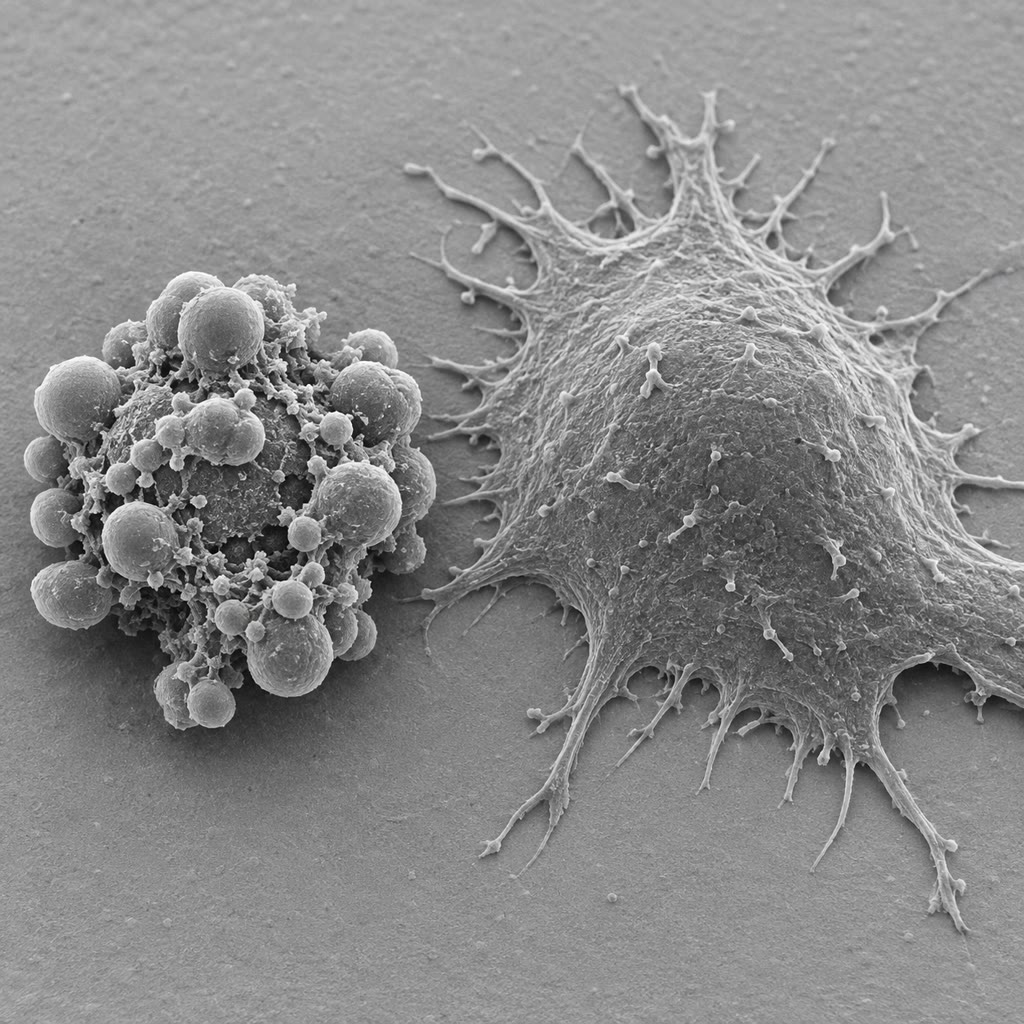
\includegraphics[width=0.40\linewidth]{images/book5/ai/b5-10-apoptotic-cell.jpg}

{\small क्रमवीक्षी इलेक्ट्रॉन सूक्ष्मदर्शी में किसी स्वस्थ कोशिका के
बगल में कोई एपॉप्टोटिक कोशिका: सिकुड़ी हुई, जिसका पृष्ठ बंद बुलबुलों
में टूट चुका है जो शोथ के किसी निशान के बिना निगल लिए जाएँगे।}
\end{omfigure}

\begin{example}[वे मृत्युएँ जो शरीर बनाती हैं]\label{ex:b3:cell-cycle-apoptosis:development}
उँगलियाँ किसी चप्पू से उनके बीच की कोशिकाओं के \omterm{def:b3:cell-cycle-apoptosis:apoptosis}{एपॉप्टोसिस} द्वारा तराशी
जाती हैं; बतख में वही कोशिकाएँ जीवित रहती हैं और झिल्ली बनी रहती है।
मेंढकछौने की पूँछ कायांतरण पर अवटु हॉर्मोन के संकेत पर सोख ली जाती है।
कशेरुकी तंत्रिका-तंत्र में बने न्यूरॉनों में से लगभग आधे जन्म से पहले
मर जाते हैं, वे जो अपने लक्ष्यों से पर्याप्त पोषी कारक नहीं पाते ---
ऐसी प्रतिस्पर्धा जो न्यूरॉनों की संख्या को उस क्षेत्र के आकार से मिला
देती है जिसकी वे सेवा करते हैं। थाइमस में बनी T~कोशिकाओं का पंचानबे
प्रतिशत वहीं मर जाता है, क्योंकि वे कुछ भी नहीं पहचानतीं या स्व को
पहचानती हैं और इसी आधार पर छाँट दी जाती हैं (\cref{ch:b3:adaptive-immunity})।
और हर दिन आंत्रीय उपकला अपनी सबसे पुरानी कोशिकाएँ रसांकुरों के सिरों पर
झाड़ देती है, त्वचा अपनी शल्कीकोशिकाएँ, रक्त अपने दिन भर जीने वाले
बूढ़े उदासीनरागी: \omterm{def:b3:cell-cycle-apoptosis:apoptosis}{एपॉप्टोसिस} ही दिनचर्या है, और ऊतक का आकार दो बड़ी
दरों का अंतर है।
\end{example}

\section{दूसरे निकास, और निकल न पाना}

\begin{definition}[नियमित परिगलन और जरावस्था]\label{def:b3:cell-cycle-apoptosis:other}
\index{नेक्रॉप्टोसिस}\index{पायरॉप्टोसिस}\index{जरावस्था}
कोशिकाओं के पास दूसरी क्रमादेशित मृत्युएँ भी हैं, और जहाँ \omterm{def:b3:cell-cycle-apoptosis:apoptosis}{एपॉप्टोसिस}
चुप है वहाँ वे सब शोथकारी हैं। \emph{नेक्रॉप्टोसिस}, जो मृत्यु
ग्राहियों से तब चलती है जब कैस्पेज़-8 रोक दी गई हो (जैसे कुछ विषाणु उसे
रोकते हैं), काइनेज़ RIPK3 को MLKL के साथ जोड़ती है, जो जीवद्रव्य-कला में
छेद कर देता है। \emph{पायरॉप्टोसिस}, जो संक्रमित महाभक्षकों में होती
है, शोथकाय (\cref{ch:b3:innate-immunity}) की कैस्पेज़-1 निष्पादित करती
है, जो गैसडर्मिन को काटकर छिद्र-कारक बनाती है और इंटरल्यूकिन-1 मुक्त
करती है। \emph{फ़ेरॉप्टोसिस} लौह-निर्भर लिपिड परॉक्सीकरण से होने वाली
मृत्यु है। कोई कोशिका बिना मरे विभाजित होना भी बंद कर सकती है:
\emph{जरावस्था} कोई स्थायी विराम है, जिसे टीलोमियर के क्षरण
(\cref{ch:b3:stem-cells}), टिकाऊ DNA क्षति या कर्कटजीन की सक्रियता के
बाद p16 और p21 थोपते हैं, और जिसमें कोशिका उपापचय की दृष्टि से सक्रिय
बनी रहती है और शोथकारी कारक स्रावित करती है। जरावस्था क्षतिग्रस्त
कोशिकाओं को विभाजनशील समूह से हटा देती है --- एक अर्बुद-दमनकारी --- और
आयु के साथ जमा होती जाती है, जहाँ उसके स्राव ऊतकों के अपह्रास में
योगदान देते हैं; चूहों में जराग्रस्त कोशिकाएँ हटाने से स्वस्थ जीवन बढ़
जाता है।
\end{definition}

\begin{remark}[बहुत कम और बहुत अधिक]\label{rem:b3:cell-cycle-apoptosis:disease}
इन कार्यक्रमों के रोग मात्रा के रोग हैं। बहुत कम मृत्यु:
कर्कट, जिसमें Bcl-2 की अति-अभिव्यक्ति या p53 के ह्रास से
एपॉप्टोटिक देहली उठ जाती है, जिससे क्षतिग्रस्त जीनोम वाली कोशिकाएँ बच
जाती हैं और और क्षति जमा करती हैं; स्व-प्रतिरक्षा, जब वे लसीकाणु बने
रहें जिन्हें छँटाई में मर जाना चाहिए था। बहुत अधिक: HIV संक्रमण में
T~कोशिकाओं का ह्रास, किसी आघात के अर्ध-क्षेत्र के न्यूरॉनों का
रक्तालपता के घंटों बाद \omterm{def:b3:cell-cycle-apoptosis:apoptosis}{एपॉप्टोसिस} से मरना (उपचार के लिए एक खिड़की),
तंत्रिका-अपह्रासी रोग में न्यूरॉनों का धीमा \omterm{def:b3:cell-cycle-apoptosis:apoptosis}{एपॉप्टोसिस}, हृदयाघात के
बाद खोई हृदय-कोशिकाएँ। कर्कट का उपचार अधिकतर उन कोशिकाओं में
\omterm{def:b3:cell-cycle-apoptosis:apoptosis}{एपॉप्टोसिस} का जान-बूझकर प्रेरण है जिनकी देहलियाँ उनके पड़ोसियों से नीची
हैं, और जो औषधें Bcl-2 तथा Cdk4/6 को लक्ष्य करती हैं वे इस अध्याय के
मानचित्रों से अभिकल्पित पहली औषधें हैं।
\end{remark}

\section{अभ्यास}

\begin{exercise}[$\star$]\label{exo:b3:cell-cycle-apoptosis:1}
चक्र की चारों प्रावस्थाएँ, हर संक्रमण को चलाने वाला चक्रिन--CDK युग्म,
और समसूत्री विभाजन को समाप्त करने वाली यूबिक्विटिन लाइगेज़ गिनाइए।
\end{exercise}

\begin{exercise}[$\star$]\label{exo:b3:cell-cycle-apoptosis:2}
इंजन की खोज में हार्टवेल, नर्स और हंट में से हर एक ने क्या योगदान दिया,
और किस जीव में?
\end{exercise}

\begin{exercise}[$\star$]\label{exo:b3:cell-cycle-apoptosis:3}
तीनों जाँच-बिंदुओं के नाम, हर एक जिस शर्त की जाँच करता है, और हर एक जिस
आणविक लक्ष्य पर काम करता है, बताइए।
\end{exercise}

\begin{exercise}[$\star$]\label{exo:b3:cell-cycle-apoptosis:4}
\omterm{def:b3:cell-cycle-apoptosis:apoptosis}{एपॉप्टोसिस} को \omterm{def:b3:cell-cycle-apoptosis:apoptosis}{परिगलन} से पाँच लक्षणों में अलग कीजिए, और \omterm{def:b3:cell-cycle-apoptosis:apoptosis}{एपॉप्टोसिस} को
निष्पादित करने वाले एंज़ाइम-वर्ग का नाम दीजिए।
\end{exercise}

\begin{exercise}[$\star\star$]\label{exo:b3:cell-cycle-apoptosis:5}
किसी मेंढक-अंडे के निष्कर्ष में \omterm{def:b3:cell-cycle-apoptosis:cdk}{चक्रिन} B $k_{s} = 1$ मात्रक प्रति
मिनट से संश्लेषित होता है; समसूत्री देहली $C_{2} = 30$ मात्रक है, निकास
देहली $C_{1} = 5$, और समसूत्री विभाजन में \omterm{def:b3:cell-cycle-apoptosis:cdk}{चक्रिन}
\qty{2}{min} के अर्ध-आयु काल से अपघटित होता है। दोलन का आवर्तकाल और
चक्र का वह अंश आँकिए जो समसूत्री विभाजन में बीतता है।
\end{exercise}

\begin{exercise}[$\star\star$]\label{exo:b3:cell-cycle-apoptosis:6}
\cref{thm:b3:cell-cycle-apoptosis:oscillator} के दोलक के रूप में किसी
ऐसी कोशिका के व्यवहार का पूर्वानुमान कीजिए जो (क) कोई अनअपघट्य
\omterm{def:b3:cell-cycle-apoptosis:cdk}{चक्रिन} B अभिव्यक्त करती है, (ख) Wee1 से वंचित है, (ग) Cdc25 से वंचित
है, (घ) ऐसा Cdk1 अभिव्यक्त करती है जिसका Wee1 फ़ॉस्फ़ोरिलन नहीं कर सकती।
\end{exercise}

\begin{exercise}[$\star\star$]\label{exo:b3:cell-cycle-apoptosis:7}
कोई राव--जॉनसन संलयन किसी G1 कोशिका और किसी S-प्रावस्था कोशिका को
जोड़ता है; दूसरा किसी G2 कोशिका और किसी S-प्रावस्था कोशिका को। हर
केंद्रक क्या करेगा, इसका पूर्वानुमान कीजिए और अनुज्ञापन तथा CDK स्तरों
से समझाइए।
\end{exercise}

\begin{exercise}[$\star\star$]\label{exo:b3:cell-cycle-apoptosis:8}
समझाइए कि \omterm{def:b3:cytoskeleton-motility:filaments}{सूक्ष्मनलिकाओं} से न जुड़ा कोई एक गुणसूत्रबिंदु पूरी कोशिका की
पश्चावस्था क्यों रोक सकता है, और ऐसी कोशिका की नियति का पूर्वानुमान
कीजिए जिसमें Mad2 विलोपित हो।
\end{exercise}

\begin{exercise}[$\star\star$]\label{exo:b3:cell-cycle-apoptosis:9}
\emph{ced-9} से वंचित; \emph{ced-3} से वंचित; दोनों से वंचित कृमि के
लक्षण-प्ररूप का पूर्वानुमान कीजिए। पथ के रूप में उपरिस्थापन समझाइए।
\end{exercise}

\begin{exercise}[$\star\star\star$]\label{exo:b3:cell-cycle-apoptosis:10}
दिखाइए कि बिना किसी द्विस्थायी स्विच के अकेला कोई ऋण पुनर्भरण पाश ---
\omterm{def:b3:cell-cycle-apoptosis:cdk}{चक्रिन} $k_{s}$ से संश्लेषित, $k_{d}AC$ से अपघटित, जिसमें $A$
बस $C$ के समानुपाती हो --- कोई स्थिर स्थायी अवस्था रखता है और दोलन
नहीं करता। S-आकार वक्र क्या जोड़ता है, और उसकी जगह कोई विलंब क्या
जोड़ता?
\end{exercise}

\begin{exercise}[$\star\star\star$]\label{exo:b3:cell-cycle-apoptosis:11}
किसी कोशिका में रक्षक Bcl-2 के $N$ अणु हैं और किसी क्षतिकारक उद्दीपन के
बाद उसे प्रति घंटा दर $r$ से BH3-मात्र संवेदक मिलते हैं, और हर संवेदक
एक रक्षक से बँधता है। समझाइए कि कोशिका लगभग समय $N/r$ पर क्यों मरती है,
चाहे उद्दीपन उससे आगे कितना ही तीव्र हो, मृत्यु अचानक क्यों होती है,
और वेनेटोक्लैक्स उस समय के साथ क्या करती है।
\end{exercise}

\begin{exercise}[$\star\star\star$]\label{exo:b3:cell-cycle-apoptosis:12}
पुटकीय लसीकार्बुद में ऐसा स्थानांतरण होता है जो \emph{BCL2} की
अति-अभिव्यक्ति करता है; कोशिकाएँ धीरे विभाजित होती हैं। दृष्टिपटलार्बुद
में \emph{RB} का ह्रास होता है; कोशिकाएँ तेज़ी से विभाजित होती हैं।
समझाइए कि हर एक अकेला घाव कोई अर्बुद कैसे पैदा करता है, पहला मंद और
दूसरा उग्र क्यों है, और हर एक इस अध्याय के दोनों कार्यक्रमों के बारे
में क्या कहता है।
\end{exercise}

\section{समस्या: किसी उपकला का जीवन और मरण}

\begin{problem}[{सप्तांत समस्या --- आंत्रीय परत कोशिका-दर-कोशिका नई की
गई, चक्र का समय चक्रिन-दोलक से निकाला गया, किसी जाँच-बिंदु की
त्रुटियाँ पूरे शरीर भर गिनी गईं, और रोज़ मरती सौ अरब कोशिकाओं का
एपॉप्टोटिक निपटान तौला गया, जिसका अंत चक्र के आवर्तकाल, प्रति दिन बनी
असुगुणित कोशिकाओं और एपॉप्टोसिस से शरीर द्वारा पुनर्चक्रित द्रव्यमान पर
होता है}]
\label{pb:b3:cell-cycle-apoptosis:1}
आँकड़े: छोटी आँत में $10^{7}$ गर्तिकाएँ हैं, और हर एक \num{3500}
कोशिकाओं का कोई रसांकुर हर $5$ दिन में नया करती है; हर गर्तिका में
लगभग $22$ स्तंभ कोशिकाएँ हैं जो दिन में एक बार विभाजित होती हैं, और
जिनकी संतति विभेदित होने से पहले $5$ बार और विभाजित होती है। दोलक:
$k_{s} = 2$ \omterm{def:b3:cell-cycle-apoptosis:cdk}{चक्रिन} मात्रक प्रति घंटा,
$C_{2} = 40$ मात्रक, $C_{1} = 8$, समसूत्री \omterm{def:b3:cell-cycle-apoptosis:cdk}{चक्रिन} का अर्ध-आयु काल
\qty{10}{min}। \omterm{def:b3:cell-cycle-apoptosis:checkpoints}{जाँच-बिंदु}: तर्कु \omterm{def:b3:cell-cycle-apoptosis:checkpoints}{जाँच-बिंदु} के बिना $50$ में एक विभाजन
कोई गुणसूत्र गलत बाँटता है; उसके साथ, \num{50000} में एक। शरीर प्रति
दिन \qty{1}{ng} द्रव्यमान की $10^{11}$ कोशिकाएँ बदलता है, और प्रोटीन
द्रव्यमान का \qty{20}{\%} है; कोई महाभक्षक \qty{1}{h} में एक एपॉप्टोटिक
कोशिका साफ़ करता है।

\medskip
\noindent\textbf{भाग I --- नवीकरण।}
\begin{enumerate}
  \item छोटी आँत प्रति दिन और प्रति सेकंड कितनी कोशिकाएँ झाड़ती है?
  \item एक गर्तिका प्रति दिन कितनी कोशिकाएँ बनाती है? जाँच: प्रति दिन
        $22$ स्तंभ विभाजन, और हर प्रतिबद्ध पुत्री $5$ बार और विभाजित
        होती हुई।
  \item यदि कोई स्तंभ कोशिका $80$ वर्षों के जीवन भर दिन में एक बार
        विभाजित हो, तो कितने विभाजन? प्रति विभाजन प्रति जीनोम $0.6$ की
        उत्परिवर्तन-दर (\cref{ch:b3:dna-repair}) के साथ वह कितने
        उत्परिवर्तन जमा करती है?
  \item संक्रमण-कोशिकाएँ हर \qty{12}{h} में विभाजित होती हैं। ऊतक तेज़,
        अल्पजीवी संक्रमण-विभाजन क्यों सह सकता है पर स्तंभ कोशिका को
        धीमा रखता है?
  \item विकिरण की कोई मात्रा सारी विभाजनशील संक्रमण-कोशिकाएँ मार देती
        है पर स्तंभ कोशिकाओं को छोड़ देती है, जो एक दिन में फिर चालू हो
        जाती हैं। बिना नई भरपाई के रसांकुर कितनी देर में नंगा हो जाएगा,
        और उसे फिर बनाने में कितना समय लगेगा? आँत विकिरण की अगेती शिकार
        क्यों है?
  \item बृहदांत्र में ऊपर की झाड़न \omterm{def:b3:cell-cycle-apoptosis:apoptosis}{एपॉप्टोसिस} से होती है (एनॉइकिस,
        यानी विलगन पर मृत्यु)। आँत के जीवाणुओं के संपर्क में रहने वाली
        किसी कोशिका के लिए यह मृत्यु-प्रकार सही क्यों है?
\end{enumerate}

\medskip
\noindent\textbf{भाग II --- घड़ी।}
\begin{enumerate}[resume]
  \item दोलक के आँकड़ों से, \omterm{def:b3:cell-cycle-apoptosis:cdk}{चक्रिन} को $C_{1}$ से $C_{2}$ तक उठने में
        कितना समय लगता है?
  \item समसूत्री अपघटन को उसे $C_{2}$ से वापस $C_{1}$ तक लाने में कितना
        समय लगता है?
  \item नंगे दोलक का आवर्तकाल, और आवर्तकाल का वह अंश जिसमें Cdk1
        सक्रिय रहता है।
  \item गर्तिका की संक्रमण-कोशिकाएँ \qty{12}{h} में चक्र लगाती हैं,
        स्तंभ कोशिकाएँ \qty{24}{h} में, मेंढक का अंडा
        \qty{30}{min} में। प्रतिरूप का कौन-सा प्राचल भिन्न है, और किसी
        कायिक कोशिका में वह अंतर कहाँ से आता है?
  \item DNA क्षति से G2/M \omterm{def:b3:cell-cycle-apoptosis:checkpoints}{जाँच-बिंदु} पर रुकी कोई कोशिका \omterm{def:b3:cell-cycle-apoptosis:cdk}{चक्रिन} B बनाती
        रहती है। वह कला-समतल पर कहाँ है, और उसे वहाँ क्या थामे रखता
        है? क्षति की मरम्मत हो जाने पर क्या होता है?
  \item कोई औषध APC/C को रोक देती है। उसकी उपस्थिति में समसूत्री विभाजन
        में प्रवेश करती किसी कोशिका की नियति बताइए।
\end{enumerate}

\medskip
\noindent\textbf{भाग III --- त्रुटियाँ।}
\begin{enumerate}[resume]
  \item $10^{11}$ कोशिकाएँ बदलने के लिए शरीर प्रति दिन कितने विभाजन
        करता है?
  \item \omterm{def:b3:cell-cycle-apoptosis:checkpoints}{जाँच-बिंदु} के साथ और उसके बिना प्रति दिन कितनी असुगुणित
        पुत्रियाँ?
  \item अधिकांश असुगुणित कोशिकाएँ मर जाती हैं या रुक जाती हैं (p53
        गलत बँटवारे पर अनुक्रिया करता है)। यदि \qty{1}{\%} बच जाएँ और
        विभाजित हों, तो जाँच-बिंदु-सक्षम कोई शरीर प्रति दिन कितनी
        असुगुणित विभाजनशील कोशिकाएँ बनाता है, और जीवन भर में कितनी?
  \item $10^{9}$ कोशिकाओं के किसी अर्बुद ने \omterm{def:b3:cell-cycle-apoptosis:checkpoints}{जाँच-बिंदु} और p53 खो दिए
        हैं। वह प्रति दिन कितने गलत बँटवारे करता है, और इससे वह तेज़ी
        से विकसित क्यों होता है?
  \item समझाइए कि तर्कु \omterm{def:b3:cell-cycle-apoptosis:checkpoints}{जाँच-बिंदु} का पूर्ण ह्रास किसी भ्रूण के लिए
        घातक क्यों है जबकि आंशिक ह्रास कर्कट को बढ़ावा देता है।
  \item डाउन संलक्षण किसी अर्धसूत्री, न कि समसूत्री, गलत बँटवारे से
        उठता है। समझाइए कि वहाँ किसी एक कोशिका की त्रुटि बच्चे की हर
        कोशिका को क्यों प्रभावित करती है, जबकि कोई एक समसूत्री त्रुटि
        एक ही वंशक्रम को प्रभावित करती है।
\end{enumerate}

\medskip
\noindent\textbf{भाग IV --- निपटान।}
\begin{enumerate}[resume]
  \item शरीर प्रति दिन और प्रति वर्ष कितने द्रव्यमान की कोशिकाएँ
        \omterm{def:b3:cell-cycle-apoptosis:apoptosis}{एपॉप्टोसिस} से निपटाता है? शरीर-द्रव्यमान से तुलना कीजिए।
  \item वह प्रति दिन कितना प्रोटीन हुआ? \qty{70}{g} के आहारी सेवन से
        तुलना कीजिए: शरीर के प्रोटीन-आवागमन का कितना अंश मरी कोशिकाओं
        का पुनर्चक्रण है?
  \item रोज़ के मुर्दे साफ़ करने के लिए लगातार काम करते कितने महाभक्षक
        चाहिए? शरीर में लगभग $10^{11}$ महाभक्षक हैं: उनके समय का कितना
        अंश?
  \item मुर्दे को लयित होने से पहले क्यों हटाना पड़ता है, और ``मुझे
        खाओ'' का संकेत कौन देता है?
  \item किसी रोगी की B~कोशिकाओं में Bcl-2 अति-अभिव्यक्त है। कौन-सा पथ
        रुका है, क्या \omterm{def:b3:cell-cycle-apoptosis:pathways}{बाह्य पथ} अब भी काम करता है, और परिणाम किसी तेज़ी
        से बढ़ते लसीकार्बुद के बजाय धीरे बढ़ता लसीकार्बुद क्यों है?
  \item किसी आघात के अर्ध-क्षेत्र के न्यूरॉन चोट के छह से चौबीस घंटे
        बाद \omterm{def:b3:cell-cycle-apoptosis:apoptosis}{एपॉप्टोसिस} से मरते हैं, और क्रोड के न्यूरॉन मिनटों में
        \omterm{def:b3:cell-cycle-apoptosis:apoptosis}{परिगलन} से। पहला उपचार के लिए खिड़की क्यों देता है और दूसरा कोई
        नहीं?
  \item सारांश दीजिए: नंगे दोलक का आवर्तकाल (प्रश्न~9), किसी सामान्य
        शरीर में प्रति दिन असुगुणित विभाजनशील कोशिकाएँ
        (प्रश्न~15), और \omterm{def:b3:cell-cycle-apoptosis:apoptosis}{एपॉप्टोसिस} से प्रति दिन पुनर्चक्रित द्रव्यमान
        (प्रश्न~19)।
\end{enumerate}
\end{problem}
